% TODO: maybe add another section about how vectorization actually works in archetypes vs types?

\section{Concurrency Model}
\label{chap:2}
The following concurrency model is of my own design. To the best of my ability I was unable to find a model like the one presented in this paper other than FLECS to a degree. Since our implementations follow similar techniques such as using archetypes and being a dense ECS, our concurrency models seem to overlap slightly but further investigation is needed.

\subsection{Formal definition} \label{section:formal_definition}
In this paper, we define an Entity Component System, short for ECS, to be a tuple $W = (T, A, \delta, \Lambda)$ consisting of:
\begin{enumerate}
    \item A finite set of types $T$
    \item A set of archetypes $A \subseteq \mathcal{P}(T)$, where $\mathcal{P}(T)$ denotes the power set of $T$    
    \item Some transition function $\delta : A \times T \rightarrow A$
    \item A set of systems $(\lambda, \lambda_{req}) \in \Lambda$ such that $\lambda : W \rightarrow W$ and $\lambda_{req} \subseteq \mathcal{P}(T)$ representing the types required to initiate $\lambda$
\end{enumerate}
This definition will be used in this chapter to generate the archetype graph.

\subsection{Types And Archetypes}
Until now, components were only stored in homogenous vectors which is great for cache locality and vectorizability but it introduces some problems -- namely with composite entities. We define a type $T$ to be the reference to a class of components. Therefore, a homogenous vector contains only components of type $T$.

\subsection{Vectorization}
Vectorization is a kind of data parallelism such that an operation is simultaneously applied to different segments of data. This is typically achieved via SIMD. Regardless, for the purpose of an ECS, vectorization means that the data needs to follow a strict standard of being contiguous in some manner. This is because of the convention that a system applies changes over components more than entities. By having archetypes be made out of components, and archetypes are able to generate a runtime Entity FSM, vectorization at the archetype level is possible. 

\subsubsection{The ABC Problem}
% https://ajmmertens.medium.com/building-an-ecs-2-archetypes-and-vectorization-fe21690805f9
The ABC Problem is a problem introduced by the FLECS creator Sander Mertens. It's a problem that demonstrates the effectiveness of Archetypes in component storage, it retains a vectorizable property, and is a good introduction to archetypes. 

Outside of ECS world $W$, suppose there exists a set of entites $E$ and $n = |E|$. Suppose $T := \{A,B,C\}$ and for each type $t \in T$, there exists a homogenous vector containing elements of type $t$. If all entities have all the components then:

\begin{figure}[H]
    \begin{lstlisting}[
        language=Java,
        numbers=none,
        style=colored
    ]
    A components[n];
    B components[n];
    C components[n];
    \end{lstlisting}
    \caption{Homogenous ECS Components}
    \label{code:homogenous_ecs}
\end{figure}

In this ideal world, entity ID can be emulated by the index to all vectors because the property $\forall t \in T : |t| = n$ holds. This ECS is positioned advantageously because all vectors are contiguous and therefore are vectorizable. This is only true because of the property mentioned.

Suppose one of the entities at some index $k$ removes some component $t$. In such a situation, the defined indexing property is broken because not all vectors are of the same length and the gap in memory now means it is impossible to write vectorized code for this ECS.

Sander Mertens uses this setup to prove that an ECS cannot vectorize homogenous components efficiently at all. This is done by reviewing all situations in which homogenous components are mutated to make vectorization impossible or difficult. By the end, he presents an alternative called archetypes and proves that archetypes leads to some form of good vectorizability.

\subsubsection{Archetypes}
Simply put, an archetype is a set of types as defined in section \ref{section:formal_definition}. Archetypes add a layer of abstraction on top of types so to make ECS queries vectorizable. Instead of creating homogenous vectors based on types in $T$, we can create homogenous vectors based on archetypes in $A$. 

\begin{figure}[H]
    \begin{lstlisting}[
        language=Java,
        numbers=none,
        style=colored
    ]
    // Type {A} "A"
    A a[A_len];
    // Type {A, B} "AB"
    A a[AB_len];
    B b[AB_len];
    // Type {A, C} "AC"
    A a[AC_len];
    C c[AC_len];
    \end{lstlisting}
    \caption{ECS Components With Archetypes $\{\{A\},\{A,B\},\{A,C\}\}$}
    \label{code:ecs_archetypes}
\end{figure}

Even though in Figure \ref{code:ecs_archetypes} those arrays are independent they do not have to be. In my implementation, for example, all components in an archetype are interleaved in a contiguous array. So essentially the papers archetypes storage looks more similar to Figure \ref{code:homogenous_ecs} than Figure \ref{code:ecs_archetypes}.

Note that since archetypes are sets of types, the archetypes $AB$ and $BA$ both represent the same archetype.

\subsection{Representing Archetypes As An Entity Finite-State-Machine}
\label{sec:fsm_arc}
ECS applications are expected to handle operations over entities that can add, modify, or remove components. In the context of archetypes, this means being able to transition an entity between archetypes. 

An example of such a situation is a game. Suppose all entities within the proximity of some point in space gain a tag component saying "buffed", but when they leave the proximity the tag component is removed. These types of state transitions may occur hundreds of times and need to be performant. 

\subsubsection{Archetype Graphs}

A finite state machine emerges from using archetypes to organize entities in a specific way. If the addition and removal of components are considered as state transitions, then the following in Figure \ref{fig:graph1} represents existing archetypes during some ECS runtime. We define vertices to be archetypes in $W$ and edges to be component addition or removal transitions to adjacent archetypes.

As an example, suppose we have an ECS with the following properties:
\begin{align}
    T &= \{A,B,C,D\} \\
    A &= \{ \emptyset, [A] , [A,C] ,[B], [A,B], [A,B,C], [B,D], [D]\} \\
    \Lambda &= \emptyset
\end{align}

\begin{figure}[htbp]
    \centering
    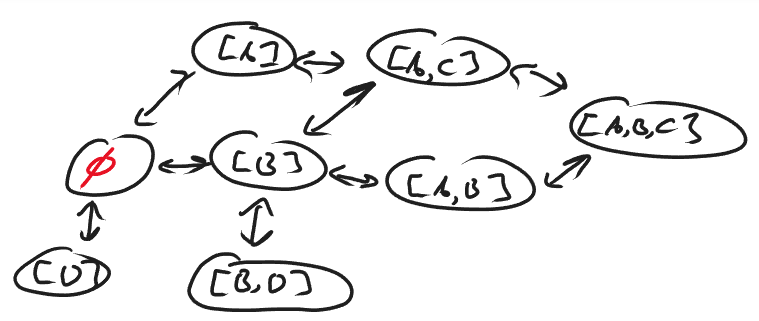
\includegraphics[width=0.5\linewidth]{resources/graph1.png}
    \caption{Example FSM Graph Of Archetypes During Runtime}
    \label{fig:graph1}
\end{figure}

As shown in Figure \ref{fig:graph1}, all graphs contain the empty set $\emptyset$ as a vertex. This is because all entities when initiated contain the the archetype with no components. As components get added to entities over their runtime, entities perform state transitions to their designated archetype. 

Archetype graphs display the following properties:

\begin{enumerate}
    \item All existing archetypes must have a path to vertex $\emptyset$.
    \item Components can appear multiple times.
    \item Archetypes can only appear once.
\end{enumerate}

There are a couple interesting things to notice in Figure \ref{fig:graph1}. Notice how there is no transition between state $[B,D]$ and $[D]$. This is because this graph represents a runtime of an ECS and while it is possible to transition between $[B,D] \leftrightarrow [D]$, it has yet to happen in this runtime. 

The component $C$ in Figure \ref{fig:graph1} is special in the regard that it is not adjacent to the $\emptyset$ vertex. This does not mean that it is impossible to create an entity with only component $C$ but that the runtime has yet to have that situation occur.

To loop back to the proximity example in section \ref{sec:fsm_arc}, by representing archetypes as runtime state transitions we can now see that large performance gains are achieved via these edges. Initially, the first entity that transitions between two states in the simulation will be slow because the edge between those two vertices must be made. Once that edge is made, it is cached and the deletion and transfer of an entity to another archetype drops from $O(N)$ to $O(1)$.

\subsubsection{Opertions On Entity FSM}
The following operations are all thread safe due to the scheduling algorithm explained in section \ref{sec:scheduling}. All implementation details are abstracted away except the operations directly done on the graph. 

\textbf{Entity Creation:} All entities when created start at the $\emptyset$ vertex. All entities that exist here are not queryable. In the papers implementation, the $\emptyset$ vertex is used as a garbage collection tool. All entities waiting for deletion are marked to transition to the empty set and cleaned at the end of the tick. 

\textbf{Entity Component Addition: } Aside from the simple transition using an existing edge. When a component addition occurs, two operations are completed. Suppose the archetype we are currently in is at archetype $G$ and are attempting to add component $C$ to transition to $G \cup \{C\}$. The two operations presented are the lookup operation and the connection operation.

\begin{enumerate}
    \item If $G \cup \{C\} \not\in A$, then do step 2. Else do step 3.
    \item Create a new archetype $G \cup \{C\} \in A$.
    \item Create the edge $G \leftrightarrow G \cup \{C\}$.
\end{enumerate}

When considering concurrency, data invalidation can occur if the archetype to transition to exists and another thread or system is using that archetype. In such a situation, the papers implemention waits for that part of the graph to be free'd.

\textbf{Entity Component Deletion: } When an entity is marked to have a component deleted. The same algorithm is used in entity component addition. Both addition and deletion use the same transition function $\delta$ of the papers ECS definition.  

\textbf{Entity Deletion: } When an entity is marked for complete deletion, the archetype it was part of must have at least one more entity to exist. If the archetype is empty, it must be removed from the graph. While this property keeps the graph mathematically pretty, there is no reason to programatically remove cached edges as they have a probability to appear again. The memory usage of an empty archetype is inconsequential. 

\subsection{Scheduling Systems}
\label{sec:scheduling}

Due to the nature of ECS patterns following some principles of data-oriented design, these architectures have an advantage in concurrency contexts. The following section is about an algorithm designed in this paper to schedule systems concurrently in such a way they produce one valid serialization point per tick. Therefore, this algorithm does not guarentee that all entities will enter a system all at once and be processed at once. Entities may be sent to the system in seemingly random orders. 

\subsubsection{Scheduling Algorithm}
The scheduling algorithm is simple. Since the entities components are currently organized into archetypes, the only points of contention are those archetypes themselves. The algorithm goes as follows:

\begin{enumerate}
    \item For each $\lambda \in \Lambda$, do the following steps 2-3:
    \item Construct the set $x = \{\forall a \in A : a \cap \lambda_{req} \not= \emptyset\}$.
    \item For each archetype in set $x$, mark that archetype.
    \item Schedule a unique thread for all archetypes.
    \item For each thread, run each system that marked this archetype.
\end{enumerate}

\textbf{Example:} The following is an example graph marked based on the algorithm above.

\begin{figure}[H]
    \centering
    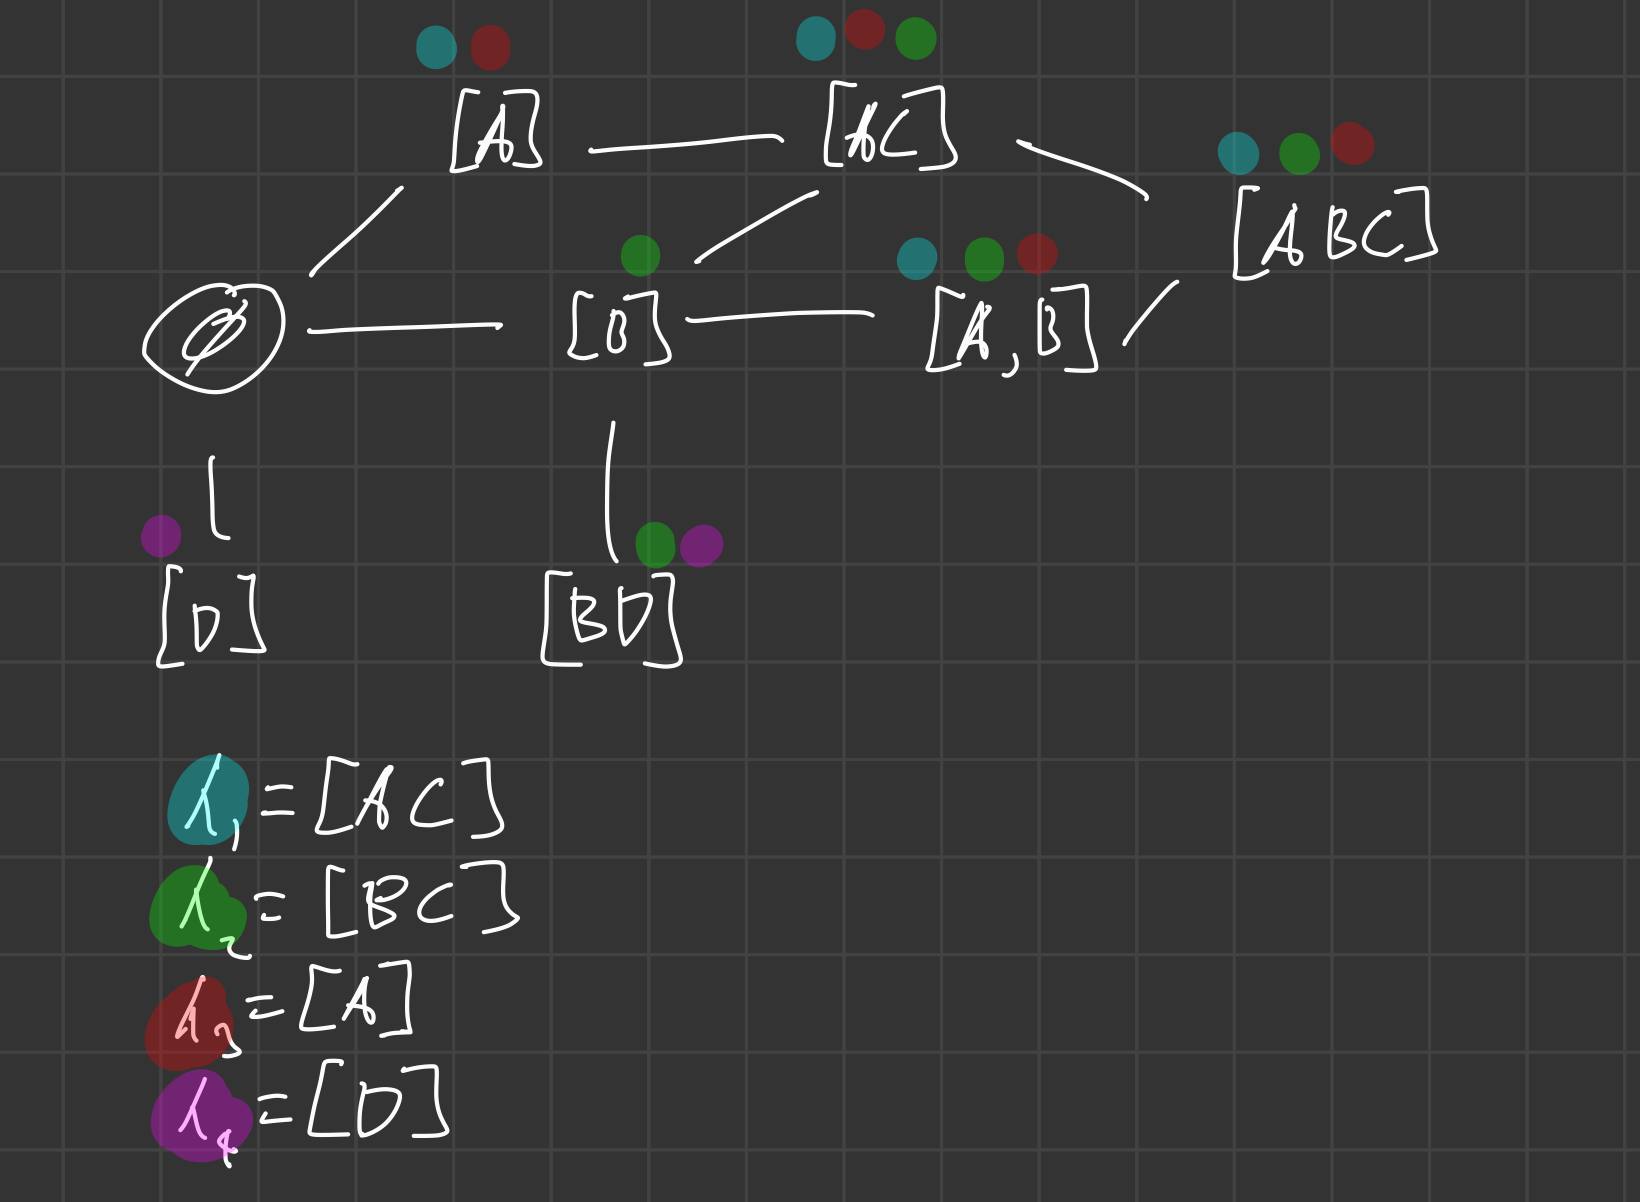
\includegraphics[width=0.5\linewidth]{resources/graph2.png}
    \caption{Example of a Scheduled Entity FSM Graph}
    \label{fig:graph2}
\end{figure}

The ECS in Figure \ref{fig:graph2} contains four systems: 

\begin{equation*}
    \Lambda = \begin{cases}
        \lambda_1 &= [A,C] \\
        \lambda_2 &= [B,C] \\ 
        \lambda_3 &= [A] \\ 
        \lambda_4 &= [D] \\ 
    \end{cases}
\end{equation*}

Notice how on any archetype vertex in this graph when there are multiple colors this signifies data contention. Depending on ECS access patterns, an ECS could possibly squeeze a bit more performance but for most cases it is unnecessary. Although, the GECS implemention does provide support for embarassingly parallel access patterns. 

\subsection{Entity Consolidation}
A key concept has been omitted thus far and that is entity consolidation. How, with these systems running concurrently, are entities transitioned between archetypes? It turns out, unlike entity modification which can be handled in parallel, component addition and deletion cannot be handled in any parallel contexts. The following sections contain a proof made for this paper and two workarounds are suggested.

\subsubsection{Entity Creation/Deletion Operations Leads To Tick Non-determinism}
\label{sec:proof1}
Suppose there exists two systems, systems A and B. The purpose of System A is to generate entities containing Component C and the purpose of System B is to consume entities that contain component C. In such an ECS runtime, that means entities are generated and transitioned to archetype $\{C\}$. Therefore the length of $\{C\}$ changes during the process of a tick. 

There are three cases in which System A and B interact:
\begin{enumerate}
    \item System A generates entities faster than B consumes
    \item System A generates entities at the same rate B consumes
    \item System A generates entities slower than B consumes
\end{enumerate}

Only in case 3 can the next tick occur. The nondeterminism introduced by allowing entity list mutations can cause program stalls such as in the manner proposed. And also in the context of a concurrent ECS, this can lead to deadlocks and livelocks.

\subsubsection{Serializability And Ledger-Based Consolidation}
In order to solve the problem of entity consolidation in any context we must fix the entity list. That means for each tick, no matter the deletion or additions performed, the entity set must stay the same until the tick is complete. As such, even if we perform perfect concurrent entity consolidation, the effort is still wasted. If the list of entities can only be mutated after the serialization point, then doing early consolidation is as if it was done now since only now can the affects of entity consolidation be seen. 

The GECS implementation proposes to use a ledger-based consolidation technique that caches mutation operations done on the entity list and applies these operations in order after the serialization point.

\subsubsection{Alternative To Ledger-Based Consolidation}
An alternative to the implementation GECS proposed is to add a constraint to $\lambda_{req}$ such that operations done where the queried archetype $a \not\subseteq \lambda_{req}$ makes them invalid. By doing so, it ensures that $\lambda$ will be scheduled by the scheduler to process $a$. 

This provides the unique opportunity that whenever working in the context of archetype $a$, all requests to create entities with archetype $a$ will be processed and all other requests ignored. In some ways, this alternative is more elegant than what GECS implemented. But this thought came too late in development and has some drawbacks. Mainly, having to know the set of components the system depends on before the system gets scheduled.

\subsubsection{$\delta$ Transition To $\emptyset$}
This case can only exist in ledger-based consolidation. Since in the alternative the system is guarenteed to run on the archetype set of a queried entity, deletion is a simple thread-safe operation. All deletion requests of entities that are not of the current archetype are ignored and deletion requests of the current archetype are accepted.

In the case of using the ledger. We must push onto the ledger that this entity is to be deleted. Before the end of the tick, we iterate and clean out all entities that are supposed to transition to $\emptyset$. 

\subsection{Parallel Processing Internal Archetypes}
There are many cases in realtime interactive systems where data is embarassingly parallel. It would be nice if there was a way for us to support embarassingly parallel operations within the ECS. An common example of an embarassingly parallel system in an ECS is applying gravity to a set of objects. Calculating the next position of an entity is an isolated operation than can be divided up to threads since there is zero data dependencies. Luckily for us, archetypes are setup to be vectorizable and requires no need of synchronizations. Therefore we can just chunk out the vector evenly to threads that are available in the thread pool.